\chapter[FM using 555]{FM using 555}

\section*{Aim}
To design and set up a frequency modulating circuit using 555.

\section*{Theory}
Frequency modulation is an analog modulation technique in which the frequency of the carrier is varied in accordance with the message signal amplitude.
Modulation index for FM is 
\begin{equation}
m= \frac{\delta f}{f_m}=\frac{frequency \ deviation}{modulating \ signal\  frequency}
\end{equation}

555 is an IC which can be used to to set up an astable multivibrator of 50\% duty cyle whose frequency is determined by externally connected RC load. \emph{(See Appendix \ref{555}})

\noindent The standard design equation for an astable mutivibrator using 555 timer IC is defined by the following equation for its time period.
\begin{equation}
T=1.38 \ RC
\end{equation}

\noindent Thus its frequency of oscillation is 
\begin{equation}
f_0 = \frac{0.72}{RC}
\end{equation}
This frequency of oscillation remains constant as long as the pin-5 is supplied with a constant voltage. If the voltage at pin-5 is varying the frequency of oscillation of the astable multivibrator also changes along with it.

Thus astable multivibrator using 555 can be used as a carrier pulse generator. The frequency of the carrier can be varied by feeding the pin-5 with message signal.
\section*{Design}
\noindent Let the carrier frequency be given by $f_c= 10 kHz$
\begin{equation}
f_c=\frac{0.72}{RC}
\end{equation}
\noindent Let $C=0.01 \mu F$
\begin{equation}
\therefore
R=\frac{0.72}{(10) (10^3)(0.01 X 10^-6)}= \ 6.8 k\Omega
\end{equation}

The amplitude of the modulationg signal should be limited by $\frac{2}{3}V_{cc}$. This is needed to avoid over modulation. The message signal should have a frequency less than 1 kHz.

The dc supply voltage of the IC, 
\begin{equation}
V_{cc}=12 V
\end{equation}
\begin{equation}
\therefore V_{m_{pp}}=\frac{2}{3}X12 V=8V
\end{equation}
\section*{Circuit Diagram}
The circuit to implement frequency modulation using 555 is shown in Figure \ref{fm555ckt}.

\begin{figure}
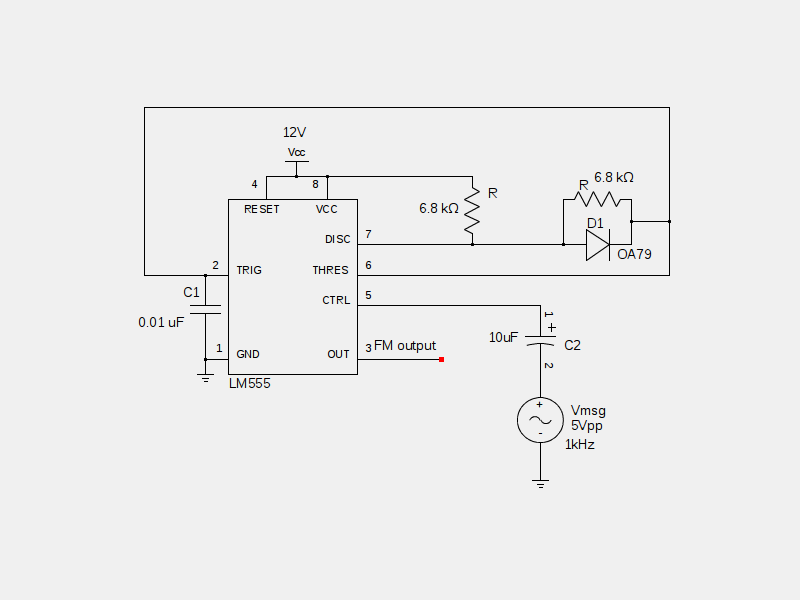
\includegraphics[height=7cm,width=\textwidth,trim=2cm 3cm 2cm 2cm,clip=true]{fm555.png}
\caption{Circuit to implement frequency modulation using 555}
\label{fm555ckt}
\end{figure}

\section*{Procedure}

\begin{itemize}
\item
Make connections as per the circuit diagram.

\item

Feed the message signal of peak-to-peak amplitude of 5V and frequency 1kHz.
\item Observe the FM output at pin number-3.

\item
Plot the observations on a graph sheet.
\end{itemize}


\section*{Observations}
Observe the input and output waveforms on a CRO and plot the same on a graph sheet. See Figure \ref{fmwaves}.


\begin{figure}
\begin{center}
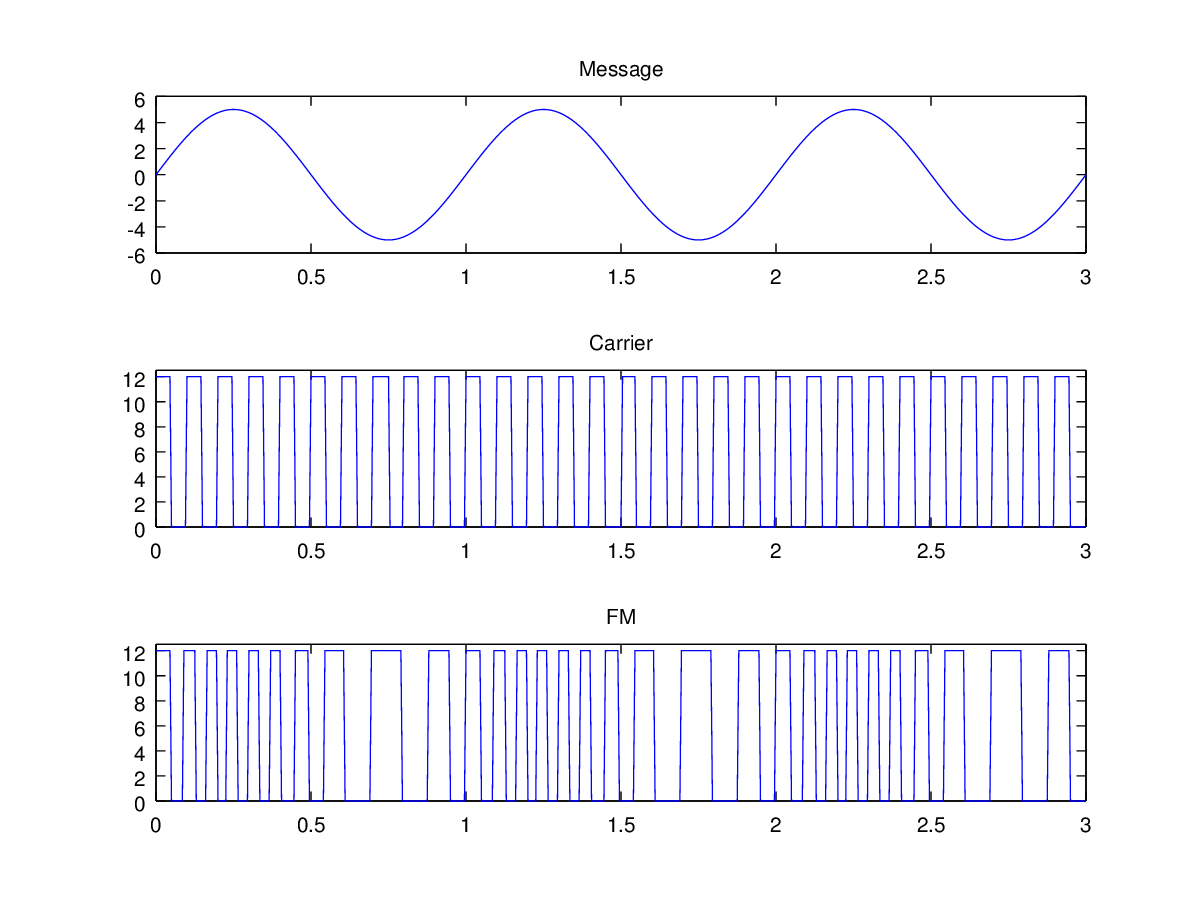
\includegraphics[height=7cm,width=10cm]{fm.png}
\caption{Message, Carrier and frequency modulated waveforms}
\label{fmwaves}
\end{center}


\end{figure}

\section*{Result}
Implemented frequency modulation of pulse carrier by sinusoidal messaage using 555 timer IC.




